\documentclass[12pt]{article}
\usepackage[T1]{fontenc}
\usepackage[latin1]{inputenc}
\usepackage[pdftex]{graphicx}
\usepackage{fancyvrb,relsize}



\title{Parallelizing Automatic Identification of Word Translations from Unrelated Corpora}
\author{Leah Hanson, Matthias Lee, Mike Weinberger}
\begin{document}
\maketitle
\begin{abstract}

Implementation of a machine translation technique which allows for learning word translations from unrelated corpora. We offer a method for scaling this technique to highly parallel graphics processors, using Python, the Python NLTK, and PyCUDA on NVIDA GPUs. We aim to highlight the advantages of using GPUs to speedup the vector calculations necessary for relating source language words to their target language counterparts.

\end{abstract}
\section{Introduction}
% Describes problem & proposed solution

With the exponential growth of technologies such as the Internet and social media, it has become easier than ever to harvest enormous monolingual datasets. There has been extensive research in the field of machine translation using parallel corpora, but little attention has been paid to learning from unrelated corpora. For the most common language pairs, parallel corpora are easy to come by. However, for lesser known languages or uncommon pairings of common languages, it may be difficult or impossible to find a sufficiently large parallel corpus. On the other hand, languages rarely lack in monolingual texts. Even uncommon pairings of common languages will have an abundance of monolingual data.

%^ it's that pairs like French-Japanese don't have much parallel data, even though they're both common.
% not just that English-"obscure tribal language" lacks data.

We based our approach on \cite{rapp1999automatic} and \cite{rapp1995identifying}. Their method depends on the notion that words tend to co-occur in similar contexts across different languages. We aimed to do two things. First, to replicate their results in a serial manner as a baseline. Second, to port their vector calculations to graphics processors with PyCUDA.
%TODO: just can't figure out how to make this listing work :(

Rapp's approach is based on building co-occurrence matrix, which keeps track of co-occurrences between words appearing within a window $w$ of one another. These matrices are computed for both the source and target language corpora and are then transformed into association matrices, by calculating the log-likelihood ratio for each co-occurrence. These association matrices/vectors can then be compared with a simple Euclidean distance metric, such as city-block distance.

Many of these calculations are embarrassingly parallel in nature and are therefore great candidates for GPU processing.


\section{Approach}
% Basic Outline
% Languages: French, German, Spanish
% Data Sources (Copuses, Base Lexicon, Test Words)
% Preprocessing
% Build Vectors
% Run tests

To resolve a basic connection between our source and target corpora we start with a base dictionary for each language pair. In this project we are aiming to expand dictionaries for English-Spanish, English-French, and English-
German. Chris Callison-Burch provided us with our base dictionaries. We preprocessed each of them to strip all multi-word translations and to only include one translation for each English word. When there were multiple translations for an English word, we picked which translation to keep at random. Next we needed to acquire four large corpora. This was done by mirroring Project Gutenberg's collection for each of the languages.

\subsection{Preprocessing}

From the dictionaries, we removed all multi-word phrases, one-to-many, and many-to-one translations to give us a simple and uniform dictionary. The caveat here is that by only keeping one translation from the one-to-many entries, we may not have chosen the best translations. Each of the dictionaries was then split it into three parts. Most of each dictionary went into a base lexicon, which was roughly 20,000 entries per language. Next, we split off roughly 5000 entries each for a test set and a development set.

We had to preprocess the Project Gutenberg books to strip out License agreements, notes, dictionaries, and unreadable characters. For each corpus, we removed some common function words (pronouns, articles, and prepositions), and then segmented the corpora into sentences and words using the Python NLTK's default splitters. Next we stemmed all the words in each corpus and in the dictionaries using the Python NLTK's SnowballStemmer for the appropriate language.

After preprocessing each corpus and dictionary, we constructed co-occurrence vectors. We cleaned and trimmed these vectors to remove noise and save memory. Each of these was then transformed into an association vector. Once we had association vectors to represent the words in each corpus, we were ready to attempt the translations.

%TODO: did we remove words that occurred fewer than 100 times? at what stage?

From the target language corpus, we pulled out the association vectors representing test words from our test dictionary. Since each of those vectors is already described in terms of words of the base lexicon, we used the base lexicon to translate each ``association word'' into English, so that the vectors would be in the same space as their English counter parts.

Next we can calculate the distance between each target language word vector and each English(source) word vector by calculating a simple Euclidean distance metric, the City-Block distance. For each foreign language word, the English word with the smallest City-Block distance is chosen as the best translation.

\subsection{Co-occurrence Counting}

The goal is to end up with a set of vectors representing the co-occurrences between all the words within our corpus. Each vector represents the context that one word (that appeared in the corpus) appeared in. This can be though of as counting how many times word A appears within some given distance $w$ from word B. Based on Rapp's research we chose $w=3$. This means that for every word B we count all words within three words of word B's position. These vectors are composed of \{word B : (word A, number)\} mappings. Each mapping represents the number of times a certain word A has co-occurred around word B within the range $w$.

As suggested by \cite{rapp1999automatic}, we also kept track of the position of word A's appearance in the window. We handled this by prefixing the mapping of each word A with its original position in context. This better captures the relation between the co-occurring words. This can be thought of as, for each of the six positions within our $w$-sized window, first generating a separate vector, and then collapsing them all into one to create a vector that is six times the size. For example, one of the six vectors would represent the words that occur two words before the target word. In practice, we just prepended each word with a number to represent which window position it was found in, so the keys of the dictionary differentiate between the positions.

\subsection{Association Vector}
% take a context vector
% prune to base lexicon
% convert values
% normalize

Turning a co-occurrence vector into an association vector is fairly straight-forward. For each vector, we remove all words that are not in our base lexicon. We do this to end up with a vector that can be fully described in terms of the relations provided by the base lexicon. At this point, we apply an optimized log-likelihood ratio formula presented in Rapp's original paper. (\emph{ see equation \ref{loglike}}). After we have calculated our association vectors, we normalize each vector to sum to one.

To convert a raw co-occurrence count into an association value, you need: the count, the total number of times the word this context vector represents was seen, the number of times this word was seen, and the total number of word tokens in the corpus.

\begin{figure}
$k_{11} =$ frequency of common occurrence of word A and word B \\
$k_{12} =$ corpus frequency of word $A - k_{11}$ \\
$k_{21} =$ corpus frequency of word $B - k_{11}$ \\
$k_{22} =$ size of corpus (in tokens) - corpus freq. of A - corpus freq. of B \\

$C_1$ = $k_{11} + k_{12}$
$C_2$ = $k_{21} + k_{22}$ \\
$R_1$ = $k_{11} + k_{21}$
$R_2$ = $k_{12} + k_{22}$ \\
$N$ = $k_{11} + k_{12} + k_{21} + k_{22}$ \\

  \begin{eqnarray*}
\sum_{i,j\in\{1,2\}} k_{ij}\log\frac{k_{ij}N}{C_iR_j} &= k_{11}\log\frac{k_{11}N}{C_1R_1} +  k_{12}\log\frac{k_{12}N}{C_1R_2} + \\
  & k_{21}\log\frac{k_{21}N}{C_2R_1} +  k_{22}\log\frac{k_{22}N}{C_2R_2} \\
  \end{eqnarray*}

  \caption{Optimized log-likelihood ratio formula.}
  \label{loglike}
\end{figure}


\subsection{Vector Similarity}

Now that we have association vectors, we can calculate the similarity between two vectors by simply calculating a ``City-Block'' distance, which is the sum of each absolute element-wise distance. (\emph{ see equation \ref{cityblock}}) To find the best translation between one of our target language test vectors and our English source vectors, we minimize on the distance between the vector pairs. We find the closest English vector to the target language vector; this is our best match and we consider it a translation.

\begin{figure}
$$\sum_{i\in U,V} |U_i - V_i| $$
\caption{City-Block distance}
  \label{cityblock}
\end{figure}

\section{Parallelizing Vector Calculations}

The parallelization effort of this project was mainly fulfilled by removing our complicated Python dictionary structures and placing our data into a flat, extremely large array which could easily be mapped to GPU memory. The main part that was outsourced to the GPU was the association vector calculation. We begin by transforming our input vectors into a 1 dimensional array which the GPU will access based on a stride(width of 1 set of variables). The actual communication with CUDA was done through the Python wrapper class called PyCUDA, which automatically compiles and interfaces with the GPU's C-based libraries.

The GPU is then set to launch as many threads as there are co-occurrence values to be calculated. This may sound inefficient, but GPU threads are extremely light weight with very little overhead. Depending on the size of the vectors being calculated, we launch close to 3.5 Million threads at once. Each block of 512 threads is mapped to 1 multiprocessor. Depending on the graphics card used to run this code, it may have between 2 and 32 of these multiprocessors, each capable of concurrently executing between 16 and 32 threads (depending on architecture).

\section{Results}

Since our results are mainly focused on the speedup gained with the same amount of processing we will mostly discuss the performance for the same operations, CPU vs GPU. The GPU executing a small test on a laptop, transforming English and German co-occurrence matrices, took 0.0004839 seconds and 0.000082015 seconds respectively. The counter part on the CPU too 0.636 seconds and 1.3375 seconds respectively. This however does not cover the full overhead of what the GPU needs to do with setup. Including this extra cost of setting up memory and copying between CPU and GPU memory, we arrive at more comparable numbers of 0.47 and 0.948 seconds respectively.

Small laptop sized tests such as mentioned above do not to the capability of the GPU justice. So we reran the same test, scaled up in size by about 8 to 10x on a workstation with a much larger, 480-core, GPU. This saw a drastic increase in performance, a test with vectors of size 756000 and 1890000, saw a GPU runtime of 0.1855seconds and 0.382seconds vs the CPU which took 5.267 seconds and 13.2501 seconds respectively. That is a 28x to 34x speedup over the CPU code. (\emph{ see figure \ref{graph}})
\begin{figure}[htb]
\centering
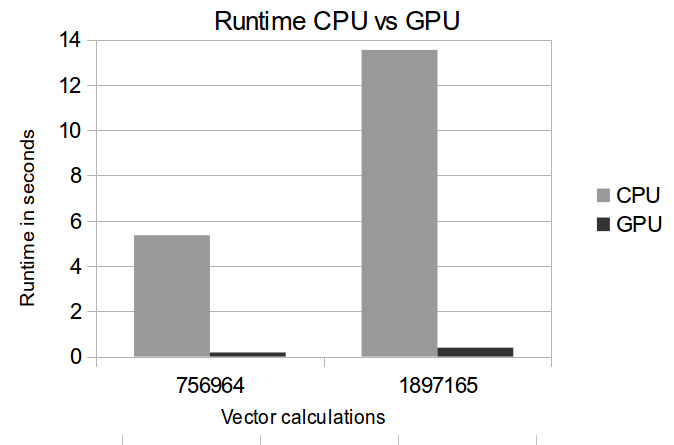
\includegraphics[scale=.5]{graph.png}
\caption{Performance CPU vs GPU runtime in seconds (lower is better)}
  \label{graph}
\end{figure}
\section{Conclusions}
We can see that the GPU outperforms the CPU implementation. However, we need to consider that we are comparing a single core CPU application against a highly parallel GPU application. If the CPU implementation were translated into C or C++ and made multi-threaded, it would be a much closer competition. Overall, the GPU will still take the lead, leaving even the fastest CPUs in the dust.

To achieve the highest efficientcy on the GPU, we would have needed to maximize the usage of GPU memory. On the Nvidia GTX480 we have 2GB of memory available, which translates into an upperbound of ~67 million vector element-pairs in memory at any given time. Maximum performance would be achieved when running closer to that limit. 

During the preprocessing stage we ran into system memory constraints, because of Pythons high memory usage during vector generation. Therefore we only used a small subset of our input data, roughly 2.5 to 3 million words depending on the language. This put to waste much of the corpora we had accumilated, German 18.5 m words, Spanish 11.25 m words, French 91.9 m words and English 1.1 b words.

We spent most of time optimizing our python processing loops which pre-preprocess(strip licenses and invalid chars) and preprocess(parse, split and stem) all of our input data. Purely by varying the way things are iterated over sometimes gained as much as 100x speedup. In the future we should attempt to also outsouce this processing to the GPU, but since everything would have to be done in C, string processing will be a nightmare. 

Overall we believe we have shown that the use of GPUs can be very adventageous and are surprised on the lack of GPU related Machine Translation literature. We will likely continue developing this in the future and have all of our source available at github.com/madmaze/parallel-mcca.

\bibliography{paper}
\bibliographystyle{plain}
\end{document}